
\section{Design Entwurf}\label{ch:DesignEntwurf}

Für das Design sollte ein Prototyp erstellt werden, der den späteren Aufbau der Applikation verdeutlicht.
Als technisches Hilfsmittel wurde das cloud-basierte Tool \textit{Figma}\footnote{\url{https://www.figma.com/}} verwendet.
Dieses bietet die Möglichkeit mit mehreren Personen in Echtzeit an einem Prototypen zu arbeiten.
Dabei ist es in seiner Bedienung leicht verständlich und bietet alle wichtigen Design-Werkzeuge. 
Außerdem können die Elemente der Benutzeroberfläche miteinander verbunden und mit Interaktionen sowie Animationen versehen werden, sodass ein interaktiver Prototyp entsteht.
Nach dem Starten eines Prototyps kann das Design der Oberfläche sowie die Navigationen geprüft werden.
Über einen generierten Link lässt sich der Prototyp mit Projektbeteiligten teilen. 

Für das Erstellen des Designs wurde eine iterative Vorgehensweise gewählt.  
Gestartet ist der Prozess mit dem Einholen von Anforderungen, siehe Kapitel \ref{ch:Anforderungsanalyse}.
Basierend darauf konnte die allgemeine Struktur der Benutzeroberfläche erstellt werden.
Anschließend verlief der Prozess in vielen Iterationsschleifen, in denen bekannte Anforderungen zunächst statisch umgesetzt und bei Rücksprachen mit den Stakeholdern deren Feedback eingeholt wurde.
Dabei wurden ebenfalls weitere Anforderungen besprochen, sodass das Design nachfolgend erweitert werden konnte.
Während den Schleifen wurde der Prototyp jeweils interaktiv erstellt, d.h. mit Animationen versehen, und es wurden weitere Details hinzugefügt.
Auf diese Weise sind während dem Projekt verschiedene Versionen des Prototyps entstanden, die jeweils mit den Stakeholdern besprochen wurden.
Neben diesen Absprachen erfolgten zusätzliche mit dem Back-End-Team.
Thema dieser Besprechungen waren die Umsetzbarkeit der Funktionalitäten, die vom Back-End bereitgestellt werden müssen.
Damit aber auch das gesamte Projektteam über den Entwurf und die Fortschritte informiert blieb, wurden das jeweils aktuelle Design in verschiedenen wöchentlichen Meetings des gesamten Teams präsentiert.
Damit jedes Team-Mitglied jederzeit auf den Prototyp zugreifen kann, wurde der Link in Trello eingetragen. 

Die designte Benutzeroberfläche besteht, wie in Abbildung \ref{fig:Seitenaufbau} dargestellt, jeweils aus drei Elementen.
Sie beinhaltet eine Kopfzeile, eine Navigationsleiste und die gewählten Inhalte.
\begin{figure}[h]
	\centering 
	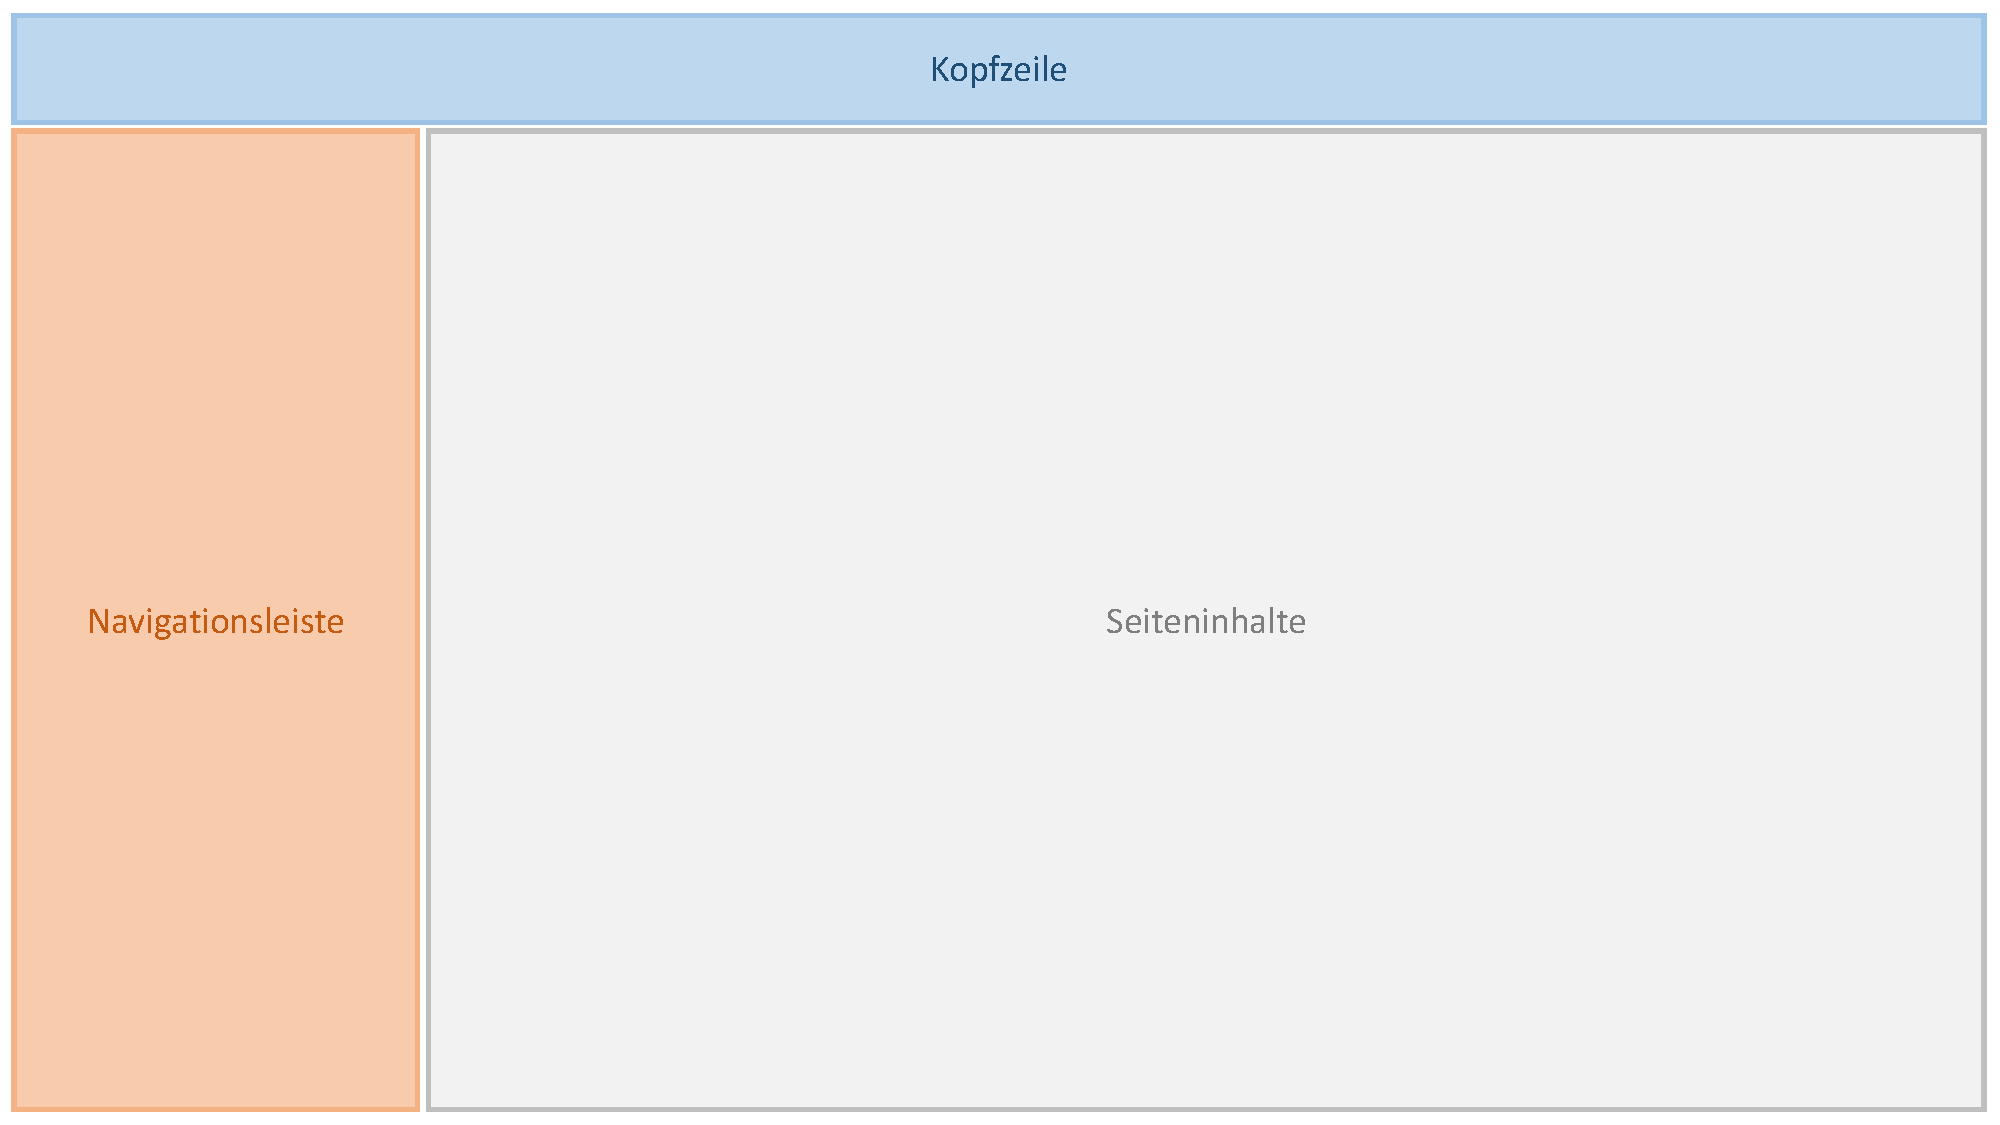
\includegraphics[width=\textwidth]{img/Seitenaufbau.pdf}
	\captionsetup{format=hang}
	\caption[Aufbau der Benutzeroberfläche]{\label{fig:Seitenaufbau}Aufbau der Benutzeroberfläche}
\end{figure}
Die Kopfzeile stellt am linken Rand das Logo der \acs{DHBW} und am rechten Rand den Benutzernamen dar.
Durch das Anklicken des Benutzernamens können allgemeine Kontoeinstellungen getätigt oder das Abmelden von der Applikation ausgelöst werden.
Auf jeder Seite der Benutzeroberfläche befindet sich außerdem am linken Rand eine vertikale Navigationsleiste.
Diese beinhaltet die vier Hauptseiten und ermöglicht das Navigieren zwischen diesen.
Es können die Vorlesungen und Vorlesungspläne je Kurs, eine Übersicht der Dozenten und verschiedene Modulkataloge angeschaut werden. Die Datenverwaltung ermöglicht das Hinzufügen, Ändern und Löschen von Studiengängen, Schwerpunkten und Prüfungsleistungen.

In Abbildung \ref{fig:Mockup} wird eine Hauptseite des Prototyps dargestellt. Das gesamte Mockup ist unter diesem \underline{\hyperlink{https://www.figma.com/proto/WZp01tmSA4nxDskhnfqv3x/Fourth-Prototype?node-id=1\%3A2\&scaling=contain}{Link}} zu finden.

\begin{figure}[H]
	\centering 
	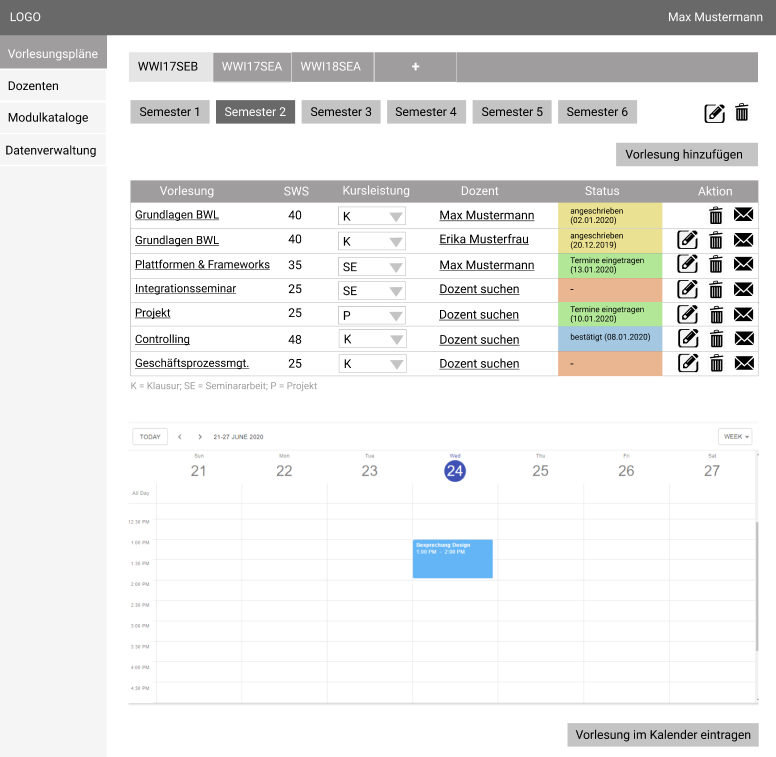
\includegraphics[width=\textwidth]{img/Mockup.PNG}
	\captionsetup{format=hang}
	\caption[Hauptseite ds Prototyps]{\label{fig:Mockup}Hauptseite des Prototyps\footnotemark}
\end{figure}
\footnotetext{\url{https://www.figma.com/proto/WZp01tmSA4nxDskhnfqv3x/Fourth-Prototype?node-id=1\%3A2\&scaling=contain}}

